\documentclass[aspectratio=169]{beamer}

\usepackage[T1]{fontenc}
\usepackage[utf8]{inputenc}
\usepackage{lmodern}
\usepackage{microtype}
\usepackage{xcolor}
\usepackage{tikz}
\usetikzlibrary{positioning, arrows.meta}
\usepackage{booktabs}
\usepackage{fontawesome5}

\definecolor{wurgreen}{HTML}{34B233}
\definecolor{darkgreen}{HTML}{1F6B1E}
\definecolor{darknavy}{HTML}{1A1A2E}
\definecolor{midgray}{HTML}{6B7280}
\definecolor{lightgray}{HTML}{F3F4F6}
\definecolor{lightgreen}{HTML}{E8F7E8}
\definecolor{bodytext}{HTML}{1F2937}
\definecolor{warnred}{HTML}{FEE2E2}
\definecolor{warnborder}{HTML}{EF4444}

\usetheme{default}
\usecolortheme{default}
\usefonttheme{professionalfonts}
\setbeamertemplate{navigation symbols}{}
\setbeamertemplate{itemize items}{\textcolor{wurgreen}{\textbullet}}
\setbeamertemplate{itemize subitem}{\textcolor{midgray}{--}}
\setbeamercolor{frametitle}{fg=white, bg=darknavy}
\setbeamerfont{frametitle}{size=\large, series=\bfseries}
\setbeamertemplate{frametitle}{%
  \begin{beamercolorbox}[wd=\paperwidth, ht=1.1cm, dp=0.2cm, leftskip=0.6cm]{frametitle}
    \usebeamerfont{frametitle}\insertframetitle
  \end{beamercolorbox}}
\setbeamercolor{background canvas}{bg=white}
\setbeamercolor{normal text}{fg=bodytext}
\setbeamertemplate{footline}{%
  \begin{beamercolorbox}[wd=\paperwidth, ht=0.4cm, dp=0.15cm]{footline}
    \hspace{0.5cm}\textcolor{midgray}{\tiny Bags, Vectors \& Transformers · Wageningen University \& Research}%
    \hfill\textcolor{midgray}{\tiny \insertframenumber}\hspace{0.4cm}
  \end{beamercolorbox}}

\begin{document}

% ── TITLE SLIDE ──────────────────────────────────────────────────────────────
{
\setbeamertemplate{footline}{}
\begin{frame}[plain]
  \begin{tikzpicture}[remember picture, overlay]
    \fill[darknavy] (current page.south west) rectangle (current page.north east);
    \fill[wurgreen] (current page.south west) rectangle
      ([xshift=0.45cm]current page.north west);
    \node[anchor=west, text=white, font=\huge\bfseries, text width=13cm]
      at ([xshift=1.1cm, yshift=1.2cm]current page.west)
      {Bags, Vectors \& Transformers};
    \node[anchor=west, text=wurgreen, font=\large, text width=12cm]
      at ([xshift=1.1cm, yshift=0.05cm]current page.west)
      {The Limits of Bag-of-Words · Day 1, Part 5};
    \node[anchor=west, text=midgray, font=\small, text width=12cm]
      at ([xshift=1.1cm, yshift=-1.5cm]current page.west)
      {Denise J. Roth, PhD Candidate\\
       Strategic Communication Group · Wageningen University \& Research};
  \end{tikzpicture}
\end{frame}
}

% ── SLIDE 1: The setup ───────────────────────────────────────────────────────
\begin{frame}{So Far, So Good --- But\ldots}
\vspace{0.3cm}
{\small Bag-of-words methods are \textbf{workhorses}: transparent, fast, and
genuinely useful. They have carried decades of social science research.
But the \textbf{simplifying assumption} that makes them work --- treating a
document as an unordered pile of word counts --- is also their \textbf{core
weakness}.}

\bigskip
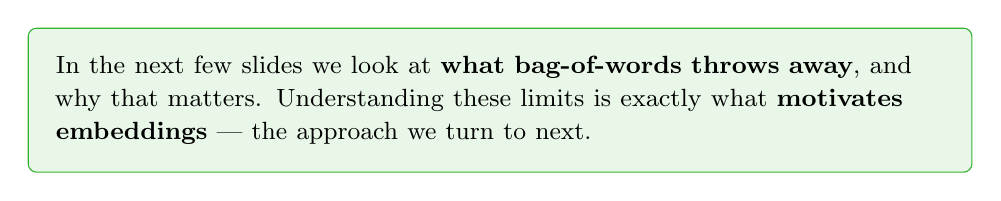
\begin{tikzpicture}
  \node[fill=lightgreen, draw=wurgreen, rounded corners=3pt,
        inner xsep=10pt, inner ysep=10pt, text width=\textwidth-24pt]{%
    {\small In the next few slides we look at \textbf{what bag-of-words throws away},
    and why that matters. Understanding these limits is exactly what \textbf{motivates
    embeddings} --- the approach we turn to next.}};
\end{tikzpicture}
\end{frame}

% ── SLIDE 2: Word order ──────────────────────────────────────────────────────
\begin{frame}{Drawback 1: Word Order Is Lost}
\vspace{0.2cm}
{\small A bag-of-words model sees only \textbf{counts}, not \textbf{sequence}.
Two sentences with the same words but opposite meaning look \textbf{identical}.}

\bigskip
\begin{columns}[T]
  \column{0.48\textwidth}
  \vspace{0pt}
  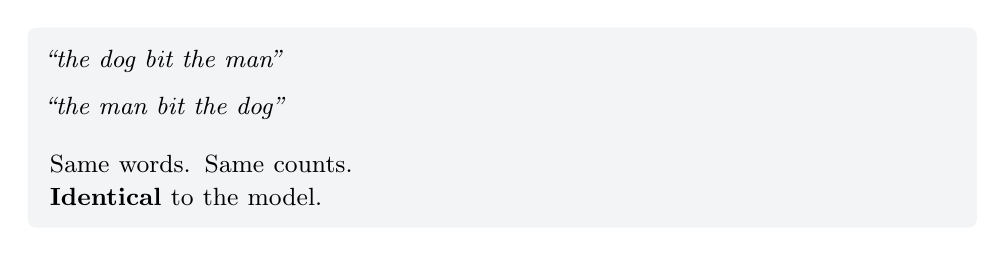
\begin{tikzpicture}
    \node[fill=lightgray, rounded corners=3pt,
          inner xsep=8pt, inner ysep=8pt, text width=\columnwidth-18pt]{%
      {\small
      \textit{``the dog bit the man''}\\[6pt]
      \textit{``the man bit the dog''}\\[10pt]
      Same words. Same counts.\\
      \textbf{Identical} to the model.}};
  \end{tikzpicture}

  \column{0.48\textwidth}
  \vspace{0pt}
  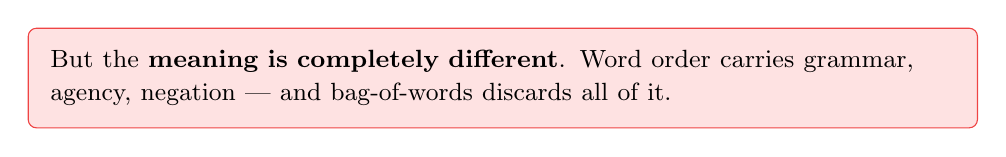
\begin{tikzpicture}
    \node[fill=warnred, draw=warnborder, rounded corners=3pt,
          inner xsep=8pt, inner ysep=8pt, text width=\columnwidth-18pt]{%
      {\small
      But the \textbf{meaning is completely different}. Word order carries
      grammar, agency, negation --- and bag-of-words discards all of it.}};
  \end{tikzpicture}
\end{columns}

\medskip
{\small\textcolor{midgray}{\textit{Partial fixes exist (n-grams capture short sequences),
but they explode the vocabulary and still miss longer-range structure.}}}
\end{frame}

% ── SLIDE 3: No semantics ────────────────────────────────────────────────────
\begin{frame}{Drawback 2: No Sense of Meaning}
\vspace{0.2cm}
{\small To a bag-of-words model, every word is a \textbf{separate, unrelated symbol}.
It has \textbf{no idea} that some words mean similar things.}

\bigskip
\begin{columns}[T]
  \column{0.48\textwidth}
  \vspace{0pt}
  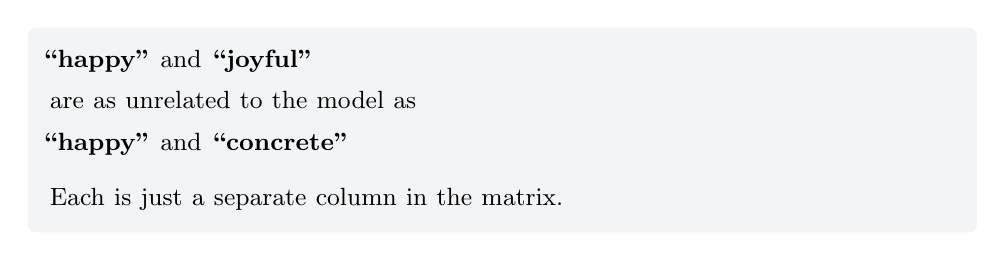
\begin{tikzpicture}
    \node[fill=lightgray, rounded corners=3pt,
          inner xsep=8pt, inner ysep=8pt, text width=\columnwidth-18pt]{%
      {\small
      \textbf{``happy''} and \textbf{``joyful''}\\[4pt]
      are as unrelated to the model as\\[4pt]
      \textbf{``happy''} and \textbf{``concrete''}\\[8pt]
      Each is just a separate column in the matrix.}};
  \end{tikzpicture}

  \column{0.48\textwidth}
  \vspace{0pt}
  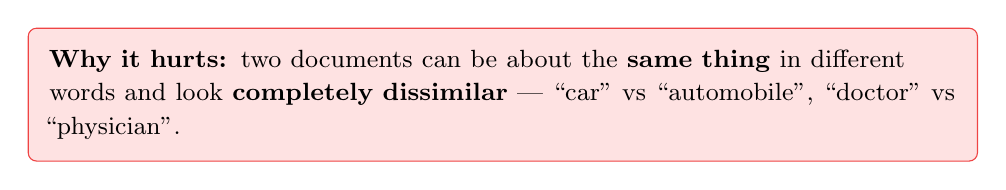
\begin{tikzpicture}
    \node[fill=warnred, draw=warnborder, rounded corners=3pt,
          inner xsep=8pt, inner ysep=8pt, text width=\columnwidth-18pt]{%
      {\small
      \textbf{Why it hurts:} two documents can be about the \textbf{same thing}
      in different words and look \textbf{completely dissimilar} ---
      ``car'' vs ``automobile'', ``doctor'' vs ``physician''.}};
  \end{tikzpicture}
\end{columns}

\medskip
{\small\textcolor{midgray}{\textit{This is the big one --- and the main gap embeddings are designed to close.}}}
\end{frame}

% ── SLIDE 4: Sparsity and dimensionality ─────────────────────────────────────
\begin{frame}{Drawback 3: High Dimensionality \& Sparsity}
\vspace{0.2cm}
{\small The document-term matrix has \textbf{one column per word} in the vocabulary.
Real corpora have \textbf{tens of thousands} of words --- so the matrix is
\textbf{enormous and mostly zeros}.}

\bigskip
\begin{columns}[T]
  \column{0.48\textwidth}
  \vspace{0pt}
  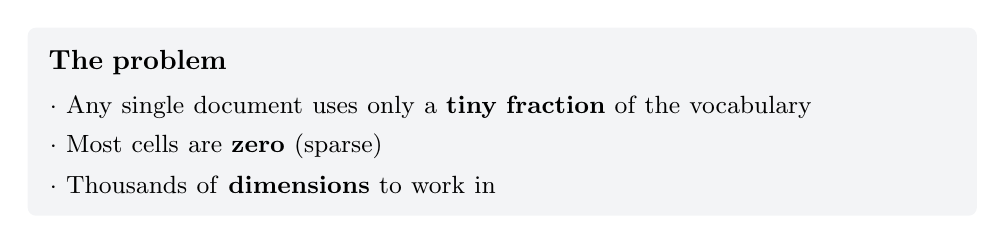
\begin{tikzpicture}
    \node[fill=lightgray, rounded corners=3pt,
          inner xsep=8pt, inner ysep=8pt, text width=\columnwidth-18pt]{%
      \textbf{The problem}\\[5pt]
      {\small
      $\cdot$ Any single document uses only a \textbf{tiny fraction} of the vocabulary\\[3pt]
      $\cdot$ Most cells are \textbf{zero} (sparse)\\[3pt]
      $\cdot$ Thousands of \textbf{dimensions} to work in}};
  \end{tikzpicture}

  \column{0.48\textwidth}
  \vspace{0pt}
  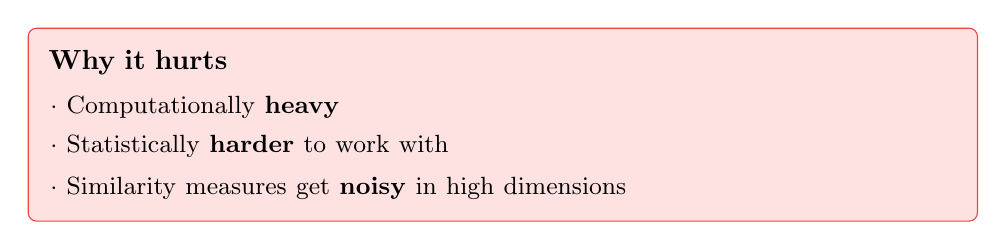
\begin{tikzpicture}
    \node[fill=warnred, draw=warnborder, rounded corners=3pt,
          inner xsep=8pt, inner ysep=8pt, text width=\columnwidth-18pt]{%
      \textbf{Why it hurts}\\[5pt]
      {\small
      $\cdot$ Computationally \textbf{heavy}\\[3pt]
      $\cdot$ Statistically \textbf{harder} to work with\\[3pt]
      $\cdot$ Similarity measures get \textbf{noisy} in high dimensions}};
  \end{tikzpicture}
\end{columns}

\medskip
{\small\textcolor{midgray}{\textit{Embeddings represent words in a few hundred \textbf{dense}
dimensions instead of tens of thousands of sparse ones.}}}
\end{frame}

% ── SLIDE 5: OOV and context ─────────────────────────────────────────────────
\begin{frame}{Drawbacks 4 \& 5: New Words \& Context}
\vspace{0.3cm}
\begin{columns}[T]
  \column{0.48\textwidth}
  \vspace{0pt}
  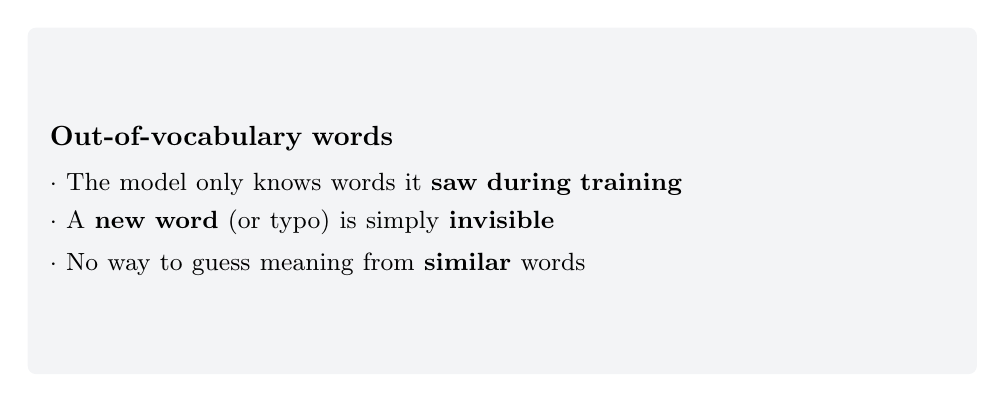
\begin{tikzpicture}
    \node[fill=lightgray, rounded corners=3pt,
          inner xsep=8pt, inner ysep=8pt, text width=\columnwidth-18pt, minimum height=4.4cm]{%
      \textbf{Out-of-vocabulary words}\\[5pt]
      {\small
      $\cdot$ The model only knows words it \textbf{saw during training}\\[3pt]
      $\cdot$ A \textbf{new word} (or typo) is simply \textbf{invisible}\\[3pt]
      $\cdot$ No way to guess meaning from \textbf{similar} words}};
  \end{tikzpicture}

  \column{0.48\textwidth}
  \vspace{0pt}
  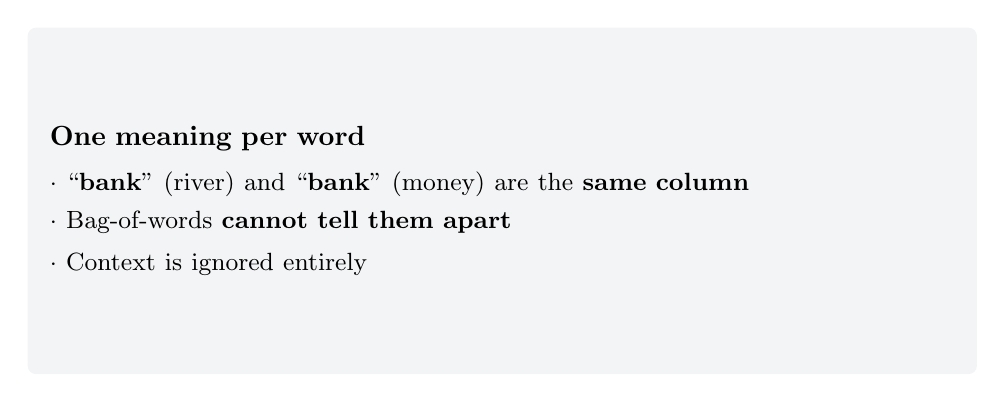
\begin{tikzpicture}
    \node[fill=lightgray, rounded corners=3pt,
          inner xsep=8pt, inner ysep=8pt, text width=\columnwidth-18pt, minimum height=4.4cm]{%
      \textbf{One meaning per word}\\[5pt]
      {\small
      $\cdot$ ``\textbf{bank}'' (river) and ``\textbf{bank}'' (money) are the \textbf{same column}\\[3pt]
      $\cdot$ Bag-of-words \textbf{cannot tell them apart}\\[3pt]
      $\cdot$ Context is ignored entirely}};
  \end{tikzpicture}
\end{columns}

\medskip
{\small\textcolor{midgray}{\textit{Static embeddings help with the first; contextual
embeddings (BERT) solve the second.}}}
\end{frame}

% ── SLIDE 6: Summary + motivate embeddings ───────────────────────────────────
\begin{frame}{Why This Points to Embeddings}
\vspace{0.2cm}
{\small Every drawback traces back to \textbf{one root problem}: bag-of-words treats
words as \textbf{isolated symbols} with no relationship to each other. What if,
instead, we could represent each word as a \textbf{position in space} --- where
\textbf{similar words sit close together}?}

\bigskip
\begin{columns}[T]
  \column{0.48\textwidth}
  \vspace{0pt}
  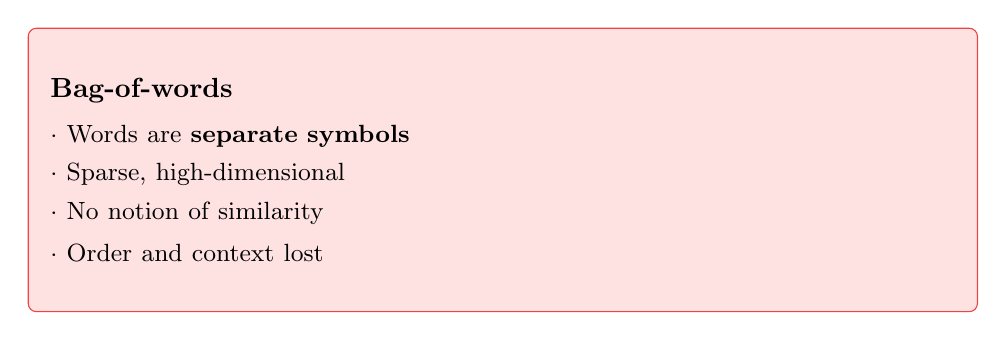
\begin{tikzpicture}
    \node[fill=warnred, draw=warnborder, rounded corners=3pt,
          inner xsep=8pt, inner ysep=8pt, text width=\columnwidth-18pt, minimum height=3.6cm]{%
      \textbf{Bag-of-words}\\[5pt]
      {\small
      $\cdot$ Words are \textbf{separate symbols}\\[3pt]
      $\cdot$ Sparse, high-dimensional\\[3pt]
      $\cdot$ No notion of similarity\\[3pt]
      $\cdot$ Order and context lost}};
  \end{tikzpicture}

  \column{0.48\textwidth}
  \vspace{0pt}
  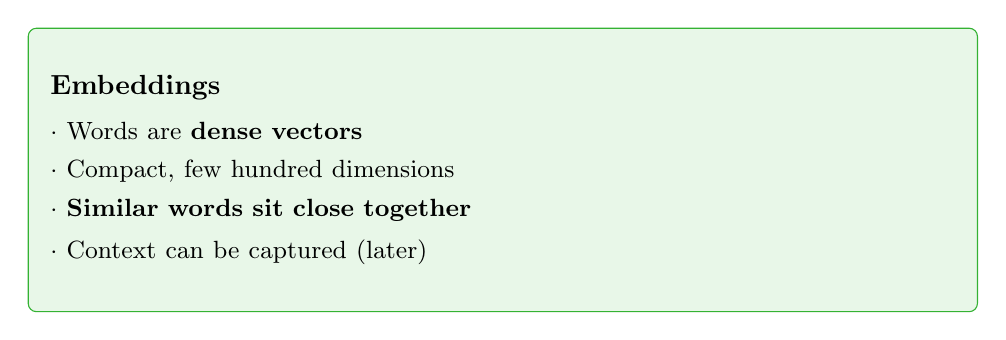
\begin{tikzpicture}
    \node[fill=lightgreen, draw=wurgreen, rounded corners=3pt,
          inner xsep=8pt, inner ysep=8pt, text width=\columnwidth-18pt, minimum height=3.6cm]{%
      \textbf{Embeddings}\\[5pt]
      {\small
      $\cdot$ Words are \textbf{dense vectors}\\[3pt]
      $\cdot$ Compact, few hundred dimensions\\[3pt]
      $\cdot$ \textbf{Similar words sit close together}\\[3pt]
      $\cdot$ Context can be captured (later)}};
  \end{tikzpicture}
\end{columns}

\medskip
{\small\textcolor{midgray}{\textit{That is exactly the idea we turn to next: word embeddings.}}}
\end{frame}

\end{document}
